Observa la gráfica de la figura \ref{fig:SINMAT1_U3_AC79_IMG1} y selecciona la opci\'on que contesta correctamente
a cada una de las siguientes preguntas:
\begin{figure}[H]
    \centering
    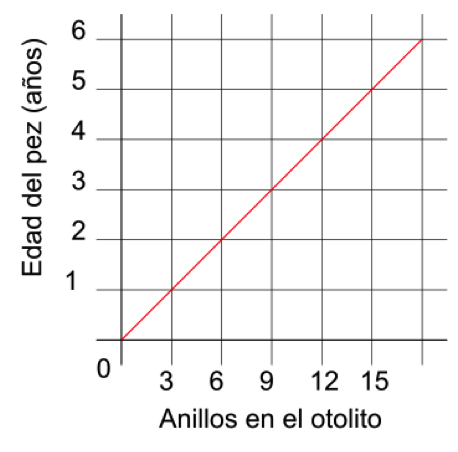
\includegraphics[width=0.35\textwidth]{../images/SINMAT1_U3_AC79_IMG1}
    \caption{Plano cartesiano con diferentes rectas distinguidas por colores.}
    \label{fig:SINMAT1_U3_AC79_IMG1}
\end{figure}
\begin{parts}
    \include*{../parts/question079a01}
    \include*{../parts/question079a02}
    \include*{../parts/question079a03}
    \include*{../parts/question079a04}
    \include*{../parts/question079a05}
    \include*{../parts/question079a06}
    \include*{../parts/question079a07}
\end{parts}